\documentclass[3p]{elsarticle}
%\documentclass[3p, twocolumn]{elsearticle}
\usepackage{amsmath}
\usepackage{amssymb}
\usepackage{gensymb}
\usepackage{upgreek}
\usepackage{float}
\parskip=0pt

\begin{document}

\begin{frontmatter}

\title{New SECM scanning algorithms for improved potentiometric imaging of circularly symmetric targets}
\cortext[cor]{Corresponding author}
\author[akiss]{Andr\'{a}s Kiss\corref{cor}}
\address[akiss, gnagy]{Department of General and Physical Chemistry, Faculty of Sciences, University of P\'{e}cs, 7624 P\'{e}cs, Ifj\'{u}s\'{a}g \'{u}tja 6, Hungary}
\address[akiss, gnagy]{J\'{a}nos Szent\'{a}gothai Research Centre, University of P\'{e}cs, 7624 P\'{e}cs, Ifj\'{u}s\'{a}g \'{u}tja 20, Hungary}
\ead{akiss@gamma.ttk.pte.hu}
\author[gnagy]{G\'{e}za Nagy}
\ead{g-nagy@gamma.ttk.pte.hu}

\begin{abstract}

To obtain high quality images in scanning probe microscopy (SPM), a certain amount of scanning time is required, depending on the number of sampling points, and the scanning speed. Usually, there is a compromise between scanning speed and image quality. This is most critical in the potentiometric scanning electrochemical microscopy (SECM), which is severely limited by the relatively long response time of the ultramicro-electrode probes. That is, scanning speed can be increased only at the expense of image quality.

In a great majority of the SECM studies, the subjects are circularly symmetric systems. In this paper, we present a method to increase SECM imaging speed of such systems, while improving image quality at the same time. It is achieved by using new, polar coordinate-based scanning patterns, exploiting the symmetry of the studied system, and using imaging time more economically. This technique, combined with our previously reported simplex algorithm for automatic target location, significantly improves the imaging of circularly symmetric targets.

Numerical simulations and SECM scans using the traditional, and the new scanning algorithms have been performed. The resulting images have been compared with the expected, ideal image.

\end{abstract}
	
\begin{keyword}
	scanning electrochemical microscope \sep potentiometry \sep response time \sep scanning algorithm
\end{keyword}
\end{frontmatter}

\section{Introduction}

Scanning electrochemical microscopy (SECM), developed by Engstrom and Bard in the eighties \cite{originalSECM, originalSECM2, originalSECM3}, is one of the many scanning probe microscopic (SPM) techniques. They all resemble the scanning tunneling microscopy (STM), the first SPM technique. Their basic component is a local experiment which, repeated at sequential locations, can be assembled to form an image \cite{stm}. This is fundamentally different from other, non-scanning microscopic techniques, such as the conventional light microscopy, where the image is instantaneous, ,,all-or-nothing''. In an SPM experiment, the time it takes to record an image depends on the number of sampling points, the distance between them, the speed at which the probe travels, the resting time before measurement, and the sampling time at a given point. In SECM, this often can be measured in tens of minutes.

The studied system is usually dynamic, and therefore image recording must be reasonably fast. If it takes too long, by the time it is completed, significant changes in the concentration profile would have already occurred. Scanning speed, however, is limited by the response time of the potentiometric cell. That is, with excessive speed, not enough time is available for the cell to reach equilibrium after advancing from one point to the next. This introduces distortion very similar to what is referred to as ,,line blur'' in imaging techniques. The resulting image will be blurred along the direction of the scanning (Figure \ref{fig:distortion}).

Potentiometric cell response time is affected by the resistance of the cell, and therefore that of the measuring electrode. Equation \ref{eq:rc} describes the relationship between cell resistance and transient cell response when the measuring electrode is brought to contact with a solution of different analyte activity.

\begin{equation}
\label{eq:rc}
	E_{cell}(t) = E_{cell}(\infty) + [E_{cell}(0) - E_{cell}(\infty)]e^{-t/RC}
\end{equation}
where $E_{cell}(t)$ is the cell potential at time $t$, $E_{cell}(\infty)$ is the equilibrium cell potential, $E_{cell}(0)$ is the cell potential prior to the change, $R$ is the resistance of the cell, and $C$ is the capacitance of the input amplifier. With decreasing electrode diameter, response time increases. With a typical ($d$ = 25 $\upmu$m) potentiometric SECM micro-electrode probe, cell resistance could reach several G$\Omega$s. Using micro-electrodes, scanning speed therefore, is a trade-off between imaging quality and scanning time.

There are several approaches to reduce SECM imaging distortion. One is decreasing the scanning speed, but then again, it compromises scanning time, and therefore temporal resolution in time-dependent studies, where multiple images must be recorded sequentially. It also introduces uncertainties during the evaluation of the image, that is, different parts of the image will belong to different instances in time. Another approach is to use SECM probes with lower resistance. Solid contact electrodes have significantly lower resistance, allowing higher scanning speed while maintaining the same image quality, or improved quality with the same scanning speed \cite{solid, spatially}.

\begin{figure}
\centering
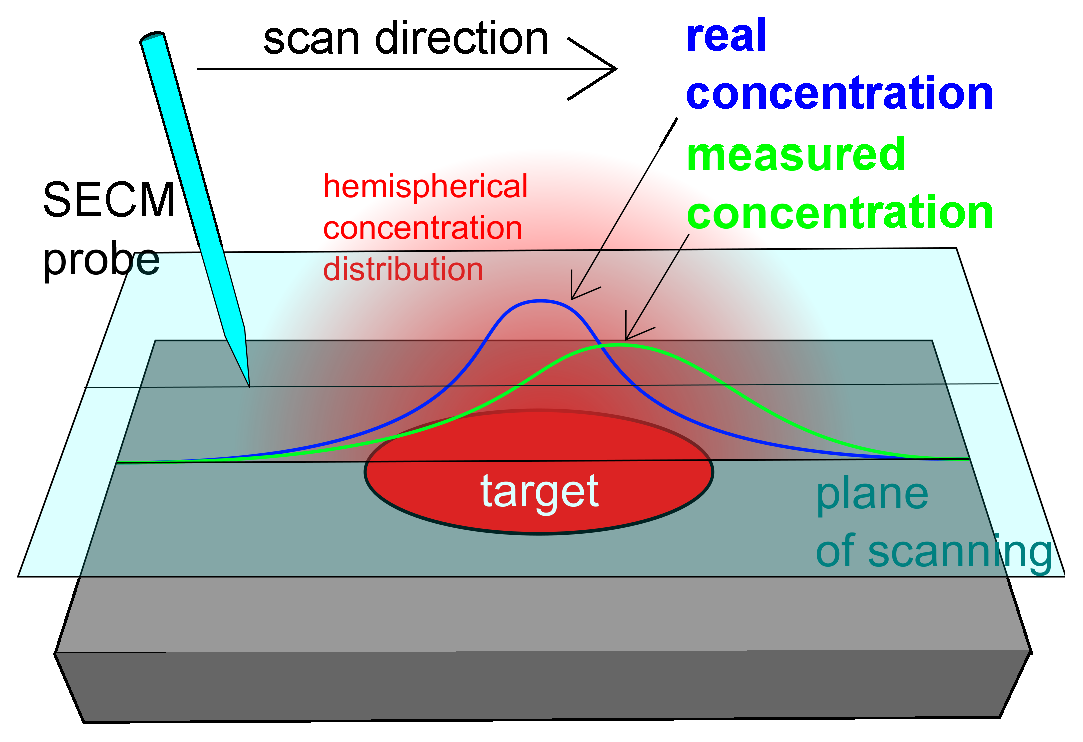
\includegraphics[width=0.5\textwidth]{distortion.eps}
\caption{The distortive effect of potentiometric SECM imaging when scanning at relatively high speed. The effective speed of the probe is too high, and therefore the time available for the potentiometric cell is too short to reach equilibrium before recording the potential at a given point. The image is blurred along the scan direction.}
\label{fig:distortion}
\end{figure}

A third approach to reduce potentiometric SECM imaging distortion, detailed in this work, is to optimize scanning algorithms. In an SECM experiment, the probe scans through a series of $X-Y$ coordinates near the area of interest, the target. To our knowledge, this always happens in the Cartesian coordinate system, using the raster scan pattern. In the 2D raster scan pattern, the image is subdivided into a sequence of parallel scan lines. The probe sweeps through every scan line, and stops periodically at the sampling points. 

There are a number of algorithms to cover all the points of a 2D raster. Three of the most common in SECM are the ,,meander'', the ,,comb'', and the ,,fast comb'' algorithms (Figure \ref{fig:patterns}). In all of these, the probe passes by the edge of the target repeatedly, where analyte concentration changes rapidly along the scan line. Advancing from one point to the next, only a certain percentage of the total change in potential can occur. Based on Equation \ref{eq:rc},

\begin{equation}
\label{eq:rc2}
	\Delta E_{cell} = [E_{cell}(i-1) - E_{cell}(i)]e^{-t/RC}
\end{equation}
where $\Delta E_{cell}$ is the observed potential change between consecutive points $i-1$ and $i$, $E_{cell}(i-1)$ and $E_{cell}(i)$ are the equilibrium potentials at those points, if $t$ is the time difference between samplings at consecutive points. Near the edge of the target, $E_{cell}(i-1)$ and $E_{cell}(i)$ can be very different, resulting a big difference between the observed and the real potential.

In this paper, we introduce new scanning patterns to improve potentiometric SECM imaging of circularly symmetric targets. They work in the common SECM setup, where the electrode is scanning in a plane parallel to the target, with a single source or a drain in the center. The target can be centered using a simplex algorithm we reported earlier \cite{simplex}. The new scanning algorithms take advantage of the circular symmetry, by scanning in concentric circles, outwards from the center. In this way, the electrode crosses the edge of the target only once. From the new algorithms, we expected improved image quality and shorter scanning time, therefore better temporal resolution in time-dependent studies.

\section{Material and methods}

\subsection{SECM scanning algorithms}
The three conventional scanning algorithms are the meander, the comb, and the fast comb. In meander, the probe travels through all of the raster coordinates without repetition and wasted movement, by alternating the $X$ scan direction from line to line, resulting in a characteristic ,,meander'' pattern. In the comb pattern, the probe sweeps through each scan line twice, back and forth, then the two scans are averaged. The fast comb algorithm scans only in one direction, and before advancing in the $Y$ direction, the probe travels back to the beginning of the scan line without measuring or stopping at all.

The two new scanning patterns proposed in this paper are called the ,,web'' and the ,,arc'' patterns. In the web pattern, sampling points are located on concentric circles with regularly increasing radius. On each circle, there are equal number of points. The first point in each circle has the angular coordinate of 0$^{o}$, which increases at regular intervals with the rest of the points. Using this pattern, resolution decreases as radius increases. The arc pattern is very similar, except that the points on the circles are separated by equally long arcs, so that with increasing radius, the number of points increases, and resolution is maintained. The scanning patterns can be seen in Figure \ref{fig:patterns}.

The images obtained with the two polar coordinate-based algorithms were interpolated to the grid points of the 2D raster used by the other algorithms to allow similar visualization.

\begin{figure}
\centering
% top left bottom right
\includegraphics[trim = 0mm 20mm 0mm 20mm, clip, width=0.25\textwidth, angle=-90]{meander_pattern.eps}\includegraphics[trim = 0mm 20mm 0mm 20mm, clip, width=0.25\textwidth, angle=-90]{fastcomb_pattern.eps}

\includegraphics[trim = 0mm 20mm 0mm 20mm, clip, width=0.25\textwidth, angle=-90]{comb_pattern.eps}\includegraphics[trim = 0mm 20mm 0mm 20mm, clip, width=0.25\textwidth, angle=-90]{web_pattern.eps}

\includegraphics[trim = 0mm 20mm 0mm 20mm, clip, width=0.25\textwidth, angle=-90]{arc_pattern.eps}
\caption{The conventional (A) meander, (B) fast comb and (C) comb, and the new, proposed (D) web, and (E) arc SECM scanning patterns for circularly symmetric targets. Red dots indicate sampling points, red line shows the probe path. Blue and green dots indicate starting and finishing positions, respectively.}
\label{fig:patterns}
\end{figure}

In the meander, fast-comb, and comb algorithms, total scanned area was 2000 $\upmu$m $\times$ 2000 $\upmu$m, resolution was 100 $\upmu$m $\times$ 100 $\upmu$m, and consequently 21 $\times$ 21 = 441 raster points altogether. In the web algorithm, the radius of the scanned area was $r$ = 1000 $\upmu$m, with $\Delta r$ = 100 $\upmu$m, and $\Delta \alpha$ = 2$\pi$/10 radians, resulting in 10 points on each circle, and a total of 110 points. In the arc pattern $r$ and $\Delta r$ was the same as in the web pattern, arc distance between adjacent points along the circles was 100 $\upmu$m, with a total of 341 points.

Both in the experimental and simulated SECM scans, for each point, 1 second was split between probe movement, resting period, and signal sampling. One measurement was performed at every point after the resting period, before positioning the probe to the next point. Probe movement speed was 312.5 $\upmu$m/s. The starting position was $x$ = -1000 $\upmu$m, $y$ = -1000 $\upmu$m, and $x$ = 0 $\upmu$m, $y$ = 0 $\upmu$m relative to the target center, for the raster-based and the polar coordinate-based algorithms, respectively.

\subsection{Model target}
To demonstrate and compare the new scanning algorithms, images of pH-dependent potential profiles were recorded $h$ = 100 $\upmu$m above a $d$ = 350 $\upmu$m graphite disc electrode, set to 2 V versus another, identical graphite electrode. At this potential difference, pH of the electrolyte will decrease at the anode, and increase at the cathode, as a consequence of water electrolysis. Both electrodes were facing upwards, embedded in an epoxy resin sleeve, with only the well-defined, disc-shaped surfaces exposed to the electrolyte. Electrolyte was unbuffered $10^{-3}$ M NaCl solution. Potential image was recorded after 10 minutes of electrolysis. During the imaging, the electrolysis cell was disconnected to avoid the electric field generated by the applied voltage affecting the image.

With a target diameter of $d$ = 350 $\upmu$m, the use of automatic target location wasn't necessary, because it could be easily centered by visual observation and manual probe positioning. Since a hemispherical concentration distribution was expected above the target, the simplex algorithm would have positioned the probe exactly above the center of the target, where the maximum concentration was expected.

\subsection{Antimony pH electrode}
To image pH-dependent potential profile, a $d$ = 50 $\upmu$m pH-sensitive antimony micro-electrode was used as SECM probe. The method of electrode preparation is described elsewhere \cite{antimony}. Electrode potential was measured against a Ag/AgCl/3M KCl reference electrode with an eDAQ pH/ISE isoPod USB (eDAQ Pty Ltd, Australia). To synchronize potentiometric signal recording and SECM probe movement, a custom software was written. A home-made SECM was used \cite{homemadeSECM}.


\section{Theory}

\subsection{Numerical simulation of diffusion from a disc source}

In potentiometric SECM, the tip is a passive probe, it does not generate or collect, therefore it does not alter the concentration profile of the species generated at the substrate. The model target can be implemented in simulation by a disk surface with a constant flux of the generated species, H$_3$O$^{+}$. Since the probe is passive, the concentration profile is only affected by the magnitude of the flux, and the diffusion coefficient of the species. The time dependent diffusion problem is described by Fick's Second Law of Diffusion:

\begin{equation}
\label{eq:fick2}
	\frac
		{\partial c}
		{\partial t}
		=
		D
		\nabla^2c
\end{equation}
where $c$ is the concentration, $t$ is time, $D$ is the diffusion coefficient. For three dimensions, Equation \ref{eq:fick2} can be expressed in discrete form for solving with the finite difference method as

\begin{equation}
\label{eq:3d}
	\begin{split}
	\frac	{c_{i,j}^{'} - c_{i,j}}{\delta t}
	=
	\frac {D} {h^2} (c_{i-1,j-1} + c_{i-1,j} + c_{i-1,j+1} + c_{i+1,j-1} + c_{i+1,j} + c_{i+1,j+1} - 6c_{i,j})
	\end{split}
\end{equation}
where $h$ is the distance between the adjacent points in space, $c_{i,j}$ is the concentration at the grid point with the coordinates of $i, j$, and $c_{i,j}^{'}$ is the same, but in the previous cycle, at the time instance $t-\delta t$. This can be solved numerically for a given time instance by iterating Equation \ref{eq:3d} on every point of a 3D matrix, which represents the diffusion system.

The simulation model consisted of a cubic diffusion field with an edge length of 20 mm, and a resolution of 10 $\upmu$m on all three axes. The top and side faces had Dirichlet boundary condition with $c$ = 0, representing the bulk solution. The bottom face had a disc shaped source with a diameter of $d$ = 350 $\upmu$m, with Neumann boundary condition, to model the graphite anode, where H$_3$O$^{+}$ was being generated. The rest of the bottom surface had Neumann boundary condition with a constant $j$ = 0 flux, modeling epoxy resin which embedded the graphite electrolysis electrode. A FORTRAN program was written to calculate the potential profile for $t$ = 600 s. A 2D section of the solved 3D diffusion matrix was taken at $h$ = 100 $\upmu$m, and it was normalized to $c_{max}$. This was the input matrix for the SECM scanning simulation.

\subsection{Simulation of the SECM scans}
The SECM scan simulations were performed on the normalized 2D section of the solved 3D diffusion matrix. The following calculation kernel was cycled through the data points using the same scanning algorithms as in the experimental SECM scans:

\begin{equation}
\label{eq:scan}
C_i = c_i + ( C_{i-1} - c_i ) \times T
\end{equation}
where $C_i$ and $c_i$ are the values of the $i$-th point in the output, and input matrices, respectively, $C_{i-1}$ is the value at the previous point, at $i-1$, and $T$ is a constant, equivalent of expression $e^{-RC/t}$ in Equation \ref{eq:rc}. A value of 0.7 was set for $T$. For $i$ = 1, $C_i$ was set to $c_i$, assuming the potentiometric cell was in equilibrium in the beginning of the scan simulation.

\section{Results and discussion}
First, SECM scanning simulations were performed and the resulting images were compared (Figure \ref{fig:simulations}). It was expected that the new, polar coordinate-based scanning algorithms would yield less distorted images than the traditional, raster-based algorithms. Not only the two new algorithms finish faster, but result images with lower distortion (Table \ref{table:comp}). Mean squared error is $9.63\times 10^{-3}$ and $2.95\times 10^{-3}$ for the images scanned with the web and the arc algorithms, respectively. In comparison, mean squared error for the images scanned with traditional meander, fast-comb, and comb algorithms are $2.75\times 10^{-2}$, $2.07\times 10^{-2}$, and $2.75\times 10^{-2}$, respectively.

Next, the experimental SECM scans were performed, with the same scanning algorithms as the simulations were. The results (Figure \ref{fig:measurements}) confirmed our presumption, that using the two new algorithms, images have less distortion, with higher similarity to the expected image.

Considering scanning time also, which are 440, 520, and 881 seconds for the meander, fast-comb, and comb algorithms, and 109, and 340 seconds for the web, and arc patterns respectively, it can be said, that the new scanning algorithms proposed in this paper shorten scanning time, and significantly improve imaging quality of circularly symmetric systems. 

There are two additional advantageous properties of the new algorithms. First, data is gathered in order of decreasing relevance, from closest to the target, to farthest from the target, without the corners of the rectangular raster patterns, which are of less importance, because of the larger distance from the target. Second, with the new algorithms, there is only positive imaging distortion (Figure \ref{fig:patterns}I, J). The observed potential, for a perfect hemispherical concentration distribution, in theory, cannot be lower above the center than the maximum value. It also cannot be higher, since the probe starts scanning in the center, where $E_{cell}(t) \approx E_{cell}(\infty)$ (Equation \ref{eq:rc}). But positive distorion can occur as the probe leaves the close vicinity of the target, advancing towards coordinates with lower concentration. This has an importance when accurate quantitative information is required about the concentration distribution above the target, such as in estimating fluxes by fitting simulation to measured images \cite{ach, co2}.

\begin{figure}
\centering
% trim = top left bottom right
\includegraphics[trim = 20mm 30mm 0mm 20mm, clip, width=0.2\textwidth, angle=-90]{meander_sim.eps} \includegraphics[trim = 20mm 30mm 0mm 20mm, clip, width=0.2\textwidth, angle=-90]{meander_delta.eps}

\includegraphics[trim = 20mm 30mm 0mm 20mm, clip, width=0.2\textwidth, angle=-90]{fastcomb_sim.eps} \includegraphics[trim = 20mm 30mm 0mm 20mm, clip, width=0.2\textwidth, angle=-90]{fastcomb_delta.eps}

\includegraphics[trim = 20mm 30mm 0mm 20mm, clip, width=0.2\textwidth, angle=-90]{comb_sim.eps} \includegraphics[trim = 20mm 30mm 0mm 20mm, clip, width=0.2\textwidth, angle=-90]{comb_delta.eps}

\includegraphics[trim = 20mm 30mm 0mm 20mm, clip, width=0.2\textwidth, angle=-90]{web_sim.eps} \includegraphics[trim = 20mm 30mm 0mm 20mm, clip, width=0.2\textwidth, angle=-90]{web_delta.eps} 

\includegraphics[trim = 20mm 30mm 0mm 20mm, clip, width=0.2\textwidth, angle=-90]{arc_sim.eps} \includegraphics[trim = 20mm 30mm 0mm 20mm, clip, width=0.2\textwidth, angle=-90]{arc_delta.eps} 

\caption{(A-E) Simulated SECM scans 100 $\upmu$m above the disc source with the meander, fast comb, comb, web, and the arc scanning algorithms, respectively. All images were normalized to the maximum concentration of the expected image (c$_{max}$). (F-J) Deviation from the expected concentration image using the meander, fast comb, comb, web, and the arc scanning algorithms, respectively. ,,$C$'' is the input (expected concentration profile), ,,$c$'' is the output (observed concentration profile) matrix for the scan simulation.}
\label{fig:simulations}
\end{figure}

\begin{figure}
\centering
\includegraphics[trim = 20mm 30mm 0mm 20mm, clip, width=0.2\textwidth, angle=-90]{meander.eps} \includegraphics[trim = 20mm 30mm 0mm 20mm, clip, width=0.2\textwidth, angle=-90]{fastcomb.eps}

\includegraphics[trim = 20mm 30mm 0mm 20mm, clip, width=0.2\textwidth, angle=-90]{comb.eps} \includegraphics[trim = 20mm 30mm 0mm 20mm, clip, width=0.2\textwidth, angle=-90]{web.eps}

\includegraphics[trim = 20mm 30mm 0mm 20mm, clip, width=0.2\textwidth, angle=-90]{arc.eps}

\caption{Experimental SECM scans 100 $\upmu$m above the disc source with the (A) meander, (B) fast comb, (C) comb, (D) web, and (E) the arc scanning algorithms. Measuring electrode was a pH-sensitive antimony micro-electrode. Potential was measured against an Ag/AgCl/3M KCl reference electrode.}
\label{fig:measurements}

\end{figure}

\begin{table}
		\caption{Comparison of the scanning algorithms.}
		\label{table:comp}
		\centering
		\begin{tabular}{r c c c}
			Algorithm & Number of sampling points & Total scan time (s) & Mean squared error \\
			\hline
			Meander & 441 & 440 & $2.75\times 10^{-2}$ \\
			Fast comb & 441 & 520  & $2.07\times 10^{-2}$ \\
			Comb & 441 & 881 & $2.75\times 10^{-2}$ \\
			Web & 110 & 109 & $9.63\times 10^{-3}$ \\
			Arc & 341 & 340 & $2.95\times 10^{-3}$ \\

		\end{tabular}

\end{table}


\section{Conclusions}
Low scanning speed is still a major limitation of potentiometric SECM. Scanning speed can be increased only at the expense of imaging quality. There are several approaches to overcome this limitation, one of which is the use of new scanning patterns, optimized for circularly symmetric systems. In this paper, we demonstrated how imaging quality and imaging speed of such systems can be improved at the same time using new, polar coordinate-based scanning algorithms. It must be noted again, that these techniques work only with circularly symmetric targets. However, a great majority of the systems studied with SECM are circularly symmetric, such as disc electrodes, anodic and cathodic sites on corroding metal surfaces, microbial colonies, pore openings. The exact position of the target must be known. To center the target, an automatic target location strategy, like our previously reported simplex algorithm can be used. 

\section{References}

\begin{thebibliography}{5}

\bibitem{originalSECM}J. Kwak, A. J. Bard, Scanning electrochemical microscopy. Theory of the feedback mode. Anal. Chem. 61.11 (1989) 1221-1227.

\bibitem{originalSECM2}A. J. Bard, F. R. F. Fan, J. Kwak, O. Lev, Scanning electrochemical microscopy. Introduction and principles. Anal. Chem. 61.2 (1989) 132-138.

\bibitem{originalSECM3}A. J. Bard, G. Denuault, Ch. Lee, D. Mandler, D. O. Wipf, Scanning electrochemical microscopy - A new technique for the characterization and modification of surfaces. Accounts. Chem. Res. 23.11 (1990) 357-363.

\bibitem{stm}H.-J. Guntherodt, R. Wiesendanger, Scanning Tunneling Microscopy I: General principles and applications to clean and adsorbate-covered surfaces. Springer-Verlag (1994).

\bibitem{solid}J. Izquierdo, A. Kiss, J. J. Santana, L. Nagy, I. Bitter, H. S. Isaacs, G. Nagy, R. M. Souto, Development of Mg2+ Ion-Selective Microelectrodes for Potentiometric Scanning Electrochemical Microscopy Monitoring of Galvanic Corrosion Processes. J. Electrochem. Soc. 160.9 (2013) C451-C459.

\bibitem{spatially}R. M. Souto, A. Kiss, J. Izquierdo, L. Nagy, I. Bitter, G. Nagy, Spatially-resolved imaging of concentration distributions on corroding magnesium-based materials exposed to aqueous environments by SECM. Electrochem. Commun. 26. (2013) 25-28.

\bibitem{simplex}B. Kovacs, B. Csoka, G. Nagy, I. Kapui, R. E. Gyurcsanyi, K. Toth, Automatic target location strategy - a novel approach in scanning electrochemical microscopy. Electroanal. 11.5 (1999) 349-355.

\bibitem{antimony}B. R. Horrocks, M. V. Mirkin, D. T. Pierce, A. J. Bard, G. Nagy, K. Toth. Scanning electrochemical microscopy. 19. Ion-selective potentiometric microscopy. Anal. Chem. 65.9 (1993) 1213-1224.

\bibitem{homemadeSECM}B. Csoka, B. Kovacs, G. Nagy, Investigation of concentration profiles inside operating biocatalytic sensors with scanning electrochemical microscopy (SECM), Biosens. Bioelectron., 18.2 (2003) 141-149.

\bibitem{ach}R. E. Gyurcsanyi, Gy. Jagerszki, G. Kiss, K. Toth, Chemical imaging of biological systems with the scanning electrochemical microscope, Bioelectrochemistry 63.1 (2004) 207-215.

\bibitem{co2}A. Kiss, L. Kiss, B. Kovacs, G. Nagy. Air Gap Microcell for Scanning Electrochemical Microscopic Imaging of Carbon Dioxide Output. Model Calculation and Gas Phase SECM Measurements for Estimation of Carbon Dioxide Producing Activity of Microbial Sources, Electroanalysis 23.10 (2011) 2320-2326.

\end{thebibliography}

\end{document}
